\documentclass{article}
\usepackage{arxiv}

\usepackage[utf8]{inputenc}
\usepackage[english, russian]{babel}
\usepackage[T1]{fontenc}
\usepackage{url}
\usepackage{booktabs}
\usepackage{amsfonts}
\usepackage{nicefrac}
\usepackage{microtype}
\usepackage{lipsum}
\usepackage{graphicx}
\usepackage{natbib}
\usepackage{doi}

\usepackage{multirow}
\usepackage{ragged2e}
\usepackage{indentfirst}
\usepackage{multicol}
\usepackage{subfig}
\usepackage{amsmath,amssymb}
\usepackage{enumerate}
\usepackage{mathtools}
\usepackage{comment}
\usepackage{multicol}

\graphicspath{ {./images/} }

\title{Детекция манипуляций в новостном потоке}

\author{ Мелихов Дмитрий Александрович \\
        Факультет вычислительной математики и кибернетики \\
        МГУ им. Ломоносова \\
        \texttt{melikhov.dmitry.a@gmail.com} \\
	%% examples of more authors
	\And
	Воронцов Константин Вячеславович \\
        Факультет вычислительной математики и кибернетики \\
        МГУ им. Ломоносова \\
        \texttt{vokov@forecsys.ru} \\
	%% \AND
	%% Coauthor \\
	%% Affiliation \\
	%% Address \\
	%% \texttt{email} \\
	%% \And
	%% Coauthor \\
	%% Affiliation \\
	%% Address \\
	%% \texttt{email} \\
	%% \And
	%% Coauthor \\
	%% Affiliation \\
	%% Address \\
	%% \texttt{email} \\
}
\date{}

\renewcommand{\shorttitle}{\textit{arXiv} Template}

%%% Add PDF metadata to help others organize their library
%%% Once the PDF is generated, you can check the metadata with
%%% $ pdfinfo template.pdf
\hypersetup{
pdftitle={A template for the arxiv style},
pdfsubject={q-bio.NC, q-bio.QM},
pdfauthor={David S.~Hippocampus, Elias D.~Striatum},
pdfkeywords={First keyword, Second keyword, More},
}

\begin{document}
\maketitle

\begin{abstract}
В работе решается задача выявления манипуляций в новостном потоке. В новостных статьях выделяются манипулятивные фрагменты и помечается тип манипуляции. Для этой задачи представляется новый набор данных на основе новостных статей из открытых сточников, где выделяются фрагменты указывающие на продвигаемые ценности. В работе рассматриваются модели на основе больших лингвистических моделей, которые выявляют фрагменты и тегируют. Для выявления фрагментов и тегирования рассматриваются постановки задачи: классификация токенов на принадлежность к фрагментуу, классификация пар токенов начало-конец. Предлагаются новые критерии качества модели, которые учитывают длину фрагментов.
\end{abstract}


\keywords{span identification \and text tagging \and manipulation detection}

\section{Введение}

Современные средства массовой информации генерируют огромный поток данных на социально-политические темы. При этом они охватывают огромное число читателей и во многом формируют у них определённый набор ценностей \cite{mutz2010mass}. Возникает потребность автоматически обрабатывать новостной поток для выявления манипуляций \cite{martino2020semeval}, суммаризации текста \cite{kemahduta2021automatic}.

Манипуляцией в тексте назвается воздействие на читателя с целью сформировать определённое отношение к цели (мишени манипуляции). Среди манипуляций можно выделить: эмоциональное воздействие, предоставление недостоверной информации, ложные причинноследственные связи.

К обработке новостного потока можно подходить с точки задачи классификации или регрессии. В 2007 году появилось соревнование SemEval-2007 Task 14 \cite{strapparava2007semeval}, где основная задача - выявление эмоциональной нагрузки заголовков статей, которая сформулирована как задача регрессии - каждой эмоции сопостовляется число от 0 до 100. В 2022 году предложили датасет на основе статей с Rappler для выявления эмоций читателя \cite{anoop22readers}.
Существует постановка задачи, в которой новости нужно классифицировать по политической идеологии, например определить кто написал статью: левый, правый или центрист. В статье \cite{bias} предлагается датасет на основе данных c сайта AllSides\footnote{\url{https://www.allsides.com/media-bias/media-bias-rating-methods}}. Также в данной статье была найдена важная проблема - смещение по источнику новости (media bias). Моделям проще выучить стиль написания статей разными СМИ и предсказывать политическую идеологию по ним, вместо того, чтобы опираться на утверждения в тексте.

Для классификации раньше использовались алгоритмы, основанные на праилах (rule based) и классические подходы. Они были популярны в соревновании SemEval-2007 Task 14 \cite{strapparava2007semeval}. С развитием нейросетей, в том числе больших языковых моделей, качество решений улучшилось. 
В 2019 году была предложена модель BERT\cite{devlin2019bert}. Данная модель стала популярной для задачи классификации текстов. В статье \cite{anoop22readers}, где предлагался новый датасет, предлагалась модель Bi-LSTM с attention усреднением эмбеддингов. В статье по предвзятости новостей \cite{bias} для классификации рассматривались LSTM и BERT.

Другой подход - выделение фрагментов (span identification)\cite{papay2020dissecting, toshniwal2020crosstask}. Выделение фрагментов используется для выделения ошибок в текст\cite{chen2020improving}, построения синтаксической структуры текста\cite{yeung2015automatic}, суммаризации \cite{Ma2018, la2019poli2sum, liu2021sent2span}, анализа цитирования научных статей\cite{la2019poli2sum}, построения графа знаний\cite{cheng2020ape}, выделение именованных сущностей\cite{li2019unified, rojas2022simple}. В задаче детекции манипуляций выделяются фрагменты, указывающие на манипуляцию. Для модерации платформ популярна задача выделения оскорбительных фрагментов. В 2021 был проведено соревнование SemEval-2021 Task 5\cite{pavlopoulos2021semeval}, где требовалось выделить оскорбительные фрагменты текста. Также проводилось соревнование на платформе codalab \footnote{https://competitions.codalab.org/competitions/36395}, результаты описаны в статье \cite{ravikiran2022findings}. В некторых постановках задач нужно сопоставлять фрагментам теги, указывающие на тип манипуляции. В 2020 году было проведено соревнование SemEval-2020 Task 11\cite{martino2020semeval}, где требуется выделять манипулятивные фрагменты и классифицировать их на 14 классов.

Для нахождения фрагментов в задаче суммаризации использовалось SVM, логистическая регрессия, решающие деревья \cite{Ma2018}, синтаксические деревья \cite{yeung2015automatic}. С развитием нейросетей стали популярны подходы с трансформерами BERT\cite{xu2023peerda}, RoBERTa\cite{ravikiran2022findings, jurkiewicz2020applicaai}, свёрточные нейронные сети \cite{dewantara-etal-2020-3218ir}, GPT-2 \cite{nouri2022data}. Данные модели можно ансамблировать и получать результат лучше, что можно заметить в обзоре результатов соревнования SemEval-2020 Task 11\cite{martino2020semeval}. Сравнение трансформерных моделей можно увидеть в статье\cite{toshniwal2020crosstask}. Также для данной задачи предобучен SpanBERT \cite{joshi2020spanbert}. Для выделения пересекающихся фрагментов можно использовать графовые нейронные сети с BERT\cite{zaratiana2022gnner}. Также для задачи с вложенными фрагментами можно использовать multiple LSTM+CRF\cite{rojas2022simple}.

\section{Постановка задачи}

В данной работе рассматривается новый русскоязычный датасет, составленный лабораторией ''Машинного обучения и семантического анализа'' института искусственного интеллекта. Для данного датасета рассматривается задачи выделения фрагментов, выделения связи между фрагментами и тегирования.

Задача выделения фрагментов - задача классификации слов:
$$
CE(S, p(S \mid \theta')) \rightarrow \min_{\theta'}
$$
Где $S \in \{B, I, O \}^{N}$ - BIO разметка текста.

Тегирование - multilabel классификация:
$$
BCE(Y, p(Y \mid \theta'')) \rightarrow \min_{\theta''}
$$
$Y_{i, j} = 1$, если фрагмент $f_i$ имеет тег $T_j$.

\section{Метод решения}

Для решения задачи упрощается структура разметки и решается сразу несколько задач:
\begin{enumerate}
  \item Нахождение фрагментов в тексте.
  \item Объедининение фрагментов в элементы разметки. Истинные фрагменты известны.
  \item Тегирование фрагментов. Истинные фрагменты известны.
  \item Тегирование элементов разметки. Истинные фрагменты и элемены разметки известны.
\end{enumerate}
Задачи решаются в одном итерационном процессе. На каждой итерации для каждой задачи последовательно делаются градиентные шаги. Подобные подходы применяются для доменной адаптации (\cite{baly2020we}).

Для вычисления эмбеддингов слов применяются лингвистические модели на основе BERT для русского языка от SberDevices(\cite{zmitrovich2023family}) и DeepPavlov(\cite{kuratov2019adaptation}). Для выявления связей между фрагментов используются text2graph модели \cite{guo2020cyclegt}. Для тегирования используются эмбеддинги фрагментов.

Находим слова, которые являются частью фрагмента.
$$
X = \{ x_n \}_{n=1}^{N} - \text{текст}~~~~~X \in \mathbb{N}^{N}
$$
$$
S \in \{0, 1, 2\}^{N} - \text{разметка фрагментов (BIO разметка)}
$$

$$
E = BERT(X) \in \mathbb{R}^{N \times d} - \text{эмбеддинги слов}
$$

$$
\hat{S}_{i, j} = \text{softmax}(E W^F)~~~~~W^F \in \mathbb{R}^{N \times 3} - \text{обучаемый параметр}
$$
1) Оптимизационная задача для выделения фрагментов:
$$
CE(S, \hat{S}) \rightarrow \min_{BERT, W^F}
$$

От структуры с элементами разметки перейдем к графу.
Матрица смежности такого графа:
$A_{i, j} = 1$, если i, j фрагменты находятся в одном элементе разметки.
Допустим, известны фрагменты
$\phi_i = \{ E_j \}_{j \in I(i)}$.
Введём преобразование, которое по эмбеддинам слов строит эмбеддинг фрагмента:
$$
F^e: \mathbb{R}^{N \times d} \rightarrow \mathbb{R}^d ~~~~~ N - \text{произвольное}
$$
$$
f_i = F^e(\phi_i) - \text{эмбеддинг i-го фрагмента}
$$
Введём близость фрагментов:
$$
s: \mathbb{R}^{2 \times d} \rightarrow [0, 1] ~~~~~\hat{A}_{i, j} = s(f_i, f_j)
$$
$s(f_i, f_j) = \sigma( \alpha f_i^T (W + W^T) f_j)$ \\
Где $\alpha, W$ - обучаемые параметры

2) Оптимизационная задача для объединения фрагментов в элемент разметки:
$$
BCE(A, \hat{A}) \rightarrow \min_{BERT, F^e, s}
$$
Задача тегирования -- задача multilabel classification. $T - $ множество тегов. Для известных фрагментов находим эмбеддинги ($f \in \mathbb{R}^{|f| \times d}$) и для них проводим классификацию:
$$
\hat{Y} = \sigma (f W^{ft})~~~~~ W^{ft} \in [0, 1]^{d \times |T|} - \text{обучаемый параметр}
$$
$$
Y \in \{0, 1\}^{|f| \times|T|} - \text{ground truth}
$$
$Y_{i, j} = 1$, если фрагмент $f_i$ имеет тег $T_j$.
3) Оптимизационная задача для тегирования фрагментов:
$$
BCE(Y, \hat{Y}) \rightarrow \min_{BERT, F^e, W^{ft}}
$$

Для аналогичного решения достаточно найти эмбеддинг элемента разметки.\\
Эмбеддинг элемента разметки можно найти по эмбеддингам фрагментов:
$$
e = E^e(elem) - \text{эмбеддинг элемента разметки}
$$
Где $elem = \{f\}$ - множество эмбеддингов фрагментов, находящихся в элементе разметки.


$$
\hat{Z} = \sigma (e W^{et})~~~~~ W^{et} \in [0, 1]^{d \times |T|} - \text{обучаемый параметр}
$$
$$
Z \in \{0, 1\}^{|e| \times|T|} - \text{ground truth}
$$
$Z_{i, j} = 1$, если элемент разметки $e_i$ имеет тег $T_j$.

4) Оптимизационная задача для тегирования элементов разметки:
$$
BCE(Z, \hat{Z}) \rightarrow \min_{BERT, F^e, E^e, W^{et}}
$$


\section{Данные}

Данные состоят из текстов новостных статей статей. Для каждого текста выделяются фрагменты, по которым можно определить каких ценностей придерживается автор. Соответсвующие ценности указываются в тегах. Фрагменты объединяются в элементы разметки. Фрагменты в элементах разметки связаны семантически, связь указывается в тегах.

\begin{figure}[h]
    \centering
    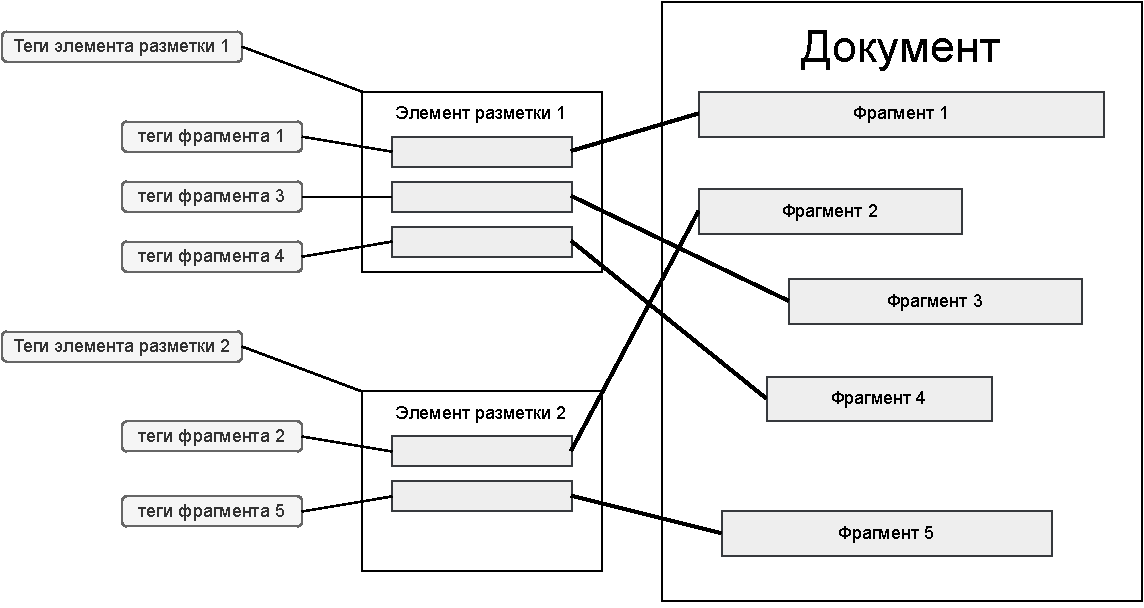
\includegraphics[width=0.95\textwidth]{markup.pdf}
\end{figure}

\section{Критерии качества модели}

Для оценки качества модели для выделения тегированных фрагментов во многих работах используется $F_1$ мера с микро усреднением. По всей выборке для каждого тега считается матрица ошибок, усредняются по тегам и считается среднее гармоническое полученных точности и полноты:
$$
TP_t = \sum_{y, \hat{y}} \sum_{i=0}^{|X|} [y_{t, i} = 1][\hat{y}_{t, i} = 1] ~~~~~~
FP_t = \sum_{y, \hat{y}} \sum_{i=0}^{|X|} [y_{t, i} = 0][\hat{y}_{t, i} = 1]
$$
$$
FN_t = \sum_{y, \hat{y}} \sum_{i=0}^{|X|} [y_{t, i} = 1][\hat{y}_{t, i} = 0]
$$
$$
TP = \frac{1}{|T|} \sum_{t \in T} TP_t~~~~~
FP = \frac{1}{|T|} \sum_{t \in T} FP_t~~~~~
FN = \frac{1}{|T|} \sum_{t \in T} FN_t
$$
$$
F_1 = \frac{2 \cdot TP}{2 \cdot TP + FP + FN}
$$
Где пара $(y, \hat{y})$ -- истинная разметка и предсказание модели.
$$
y_{t, i} = 1 \Rightarrow \text{i-е слово принадлежит фрагменту, помеченному тегом t}.
$$

\section{Эксперименты}



\bibliographystyle{unsrtnat}
\bibliography{references}

\end{document}